\chapter{Исследовательская часть}

\section{Интерфейс приложения}

На рисункaх  \ref{fig:интерфейс} -- \ref{fig:график} приведено изображение интерфейса экранов приложения.

\begin{figure}[h!]
	\centering{
\includegraphics[scale=0.28]{img/интерфейс.jpg}}
	\caption{Интерфейс}
	\label{fig:интерфейс}
\end{figure}


Главный экран приложения дает возможность ввести две матрицы, произведение которых будет вычисляться, а также предоставляется выбор метода, с помощью которого оно будет найдено. Также предусмотрена возможность сгенерировать матрицу: для этого необходимо задать размеры матриц в специальных текстовых полях и нажать на кнопку <<Генерация>>. При нажатии на кнопку <<Рассчитать>>, появляется второй экран, отображающий результирующую матрицу. При нажатии на кнопку <<График>>, находящуюся на втором экране, отображается график зависимости времени (в секундах) от количества произведенных операций.


\begin{figure}[h!]
	\centering{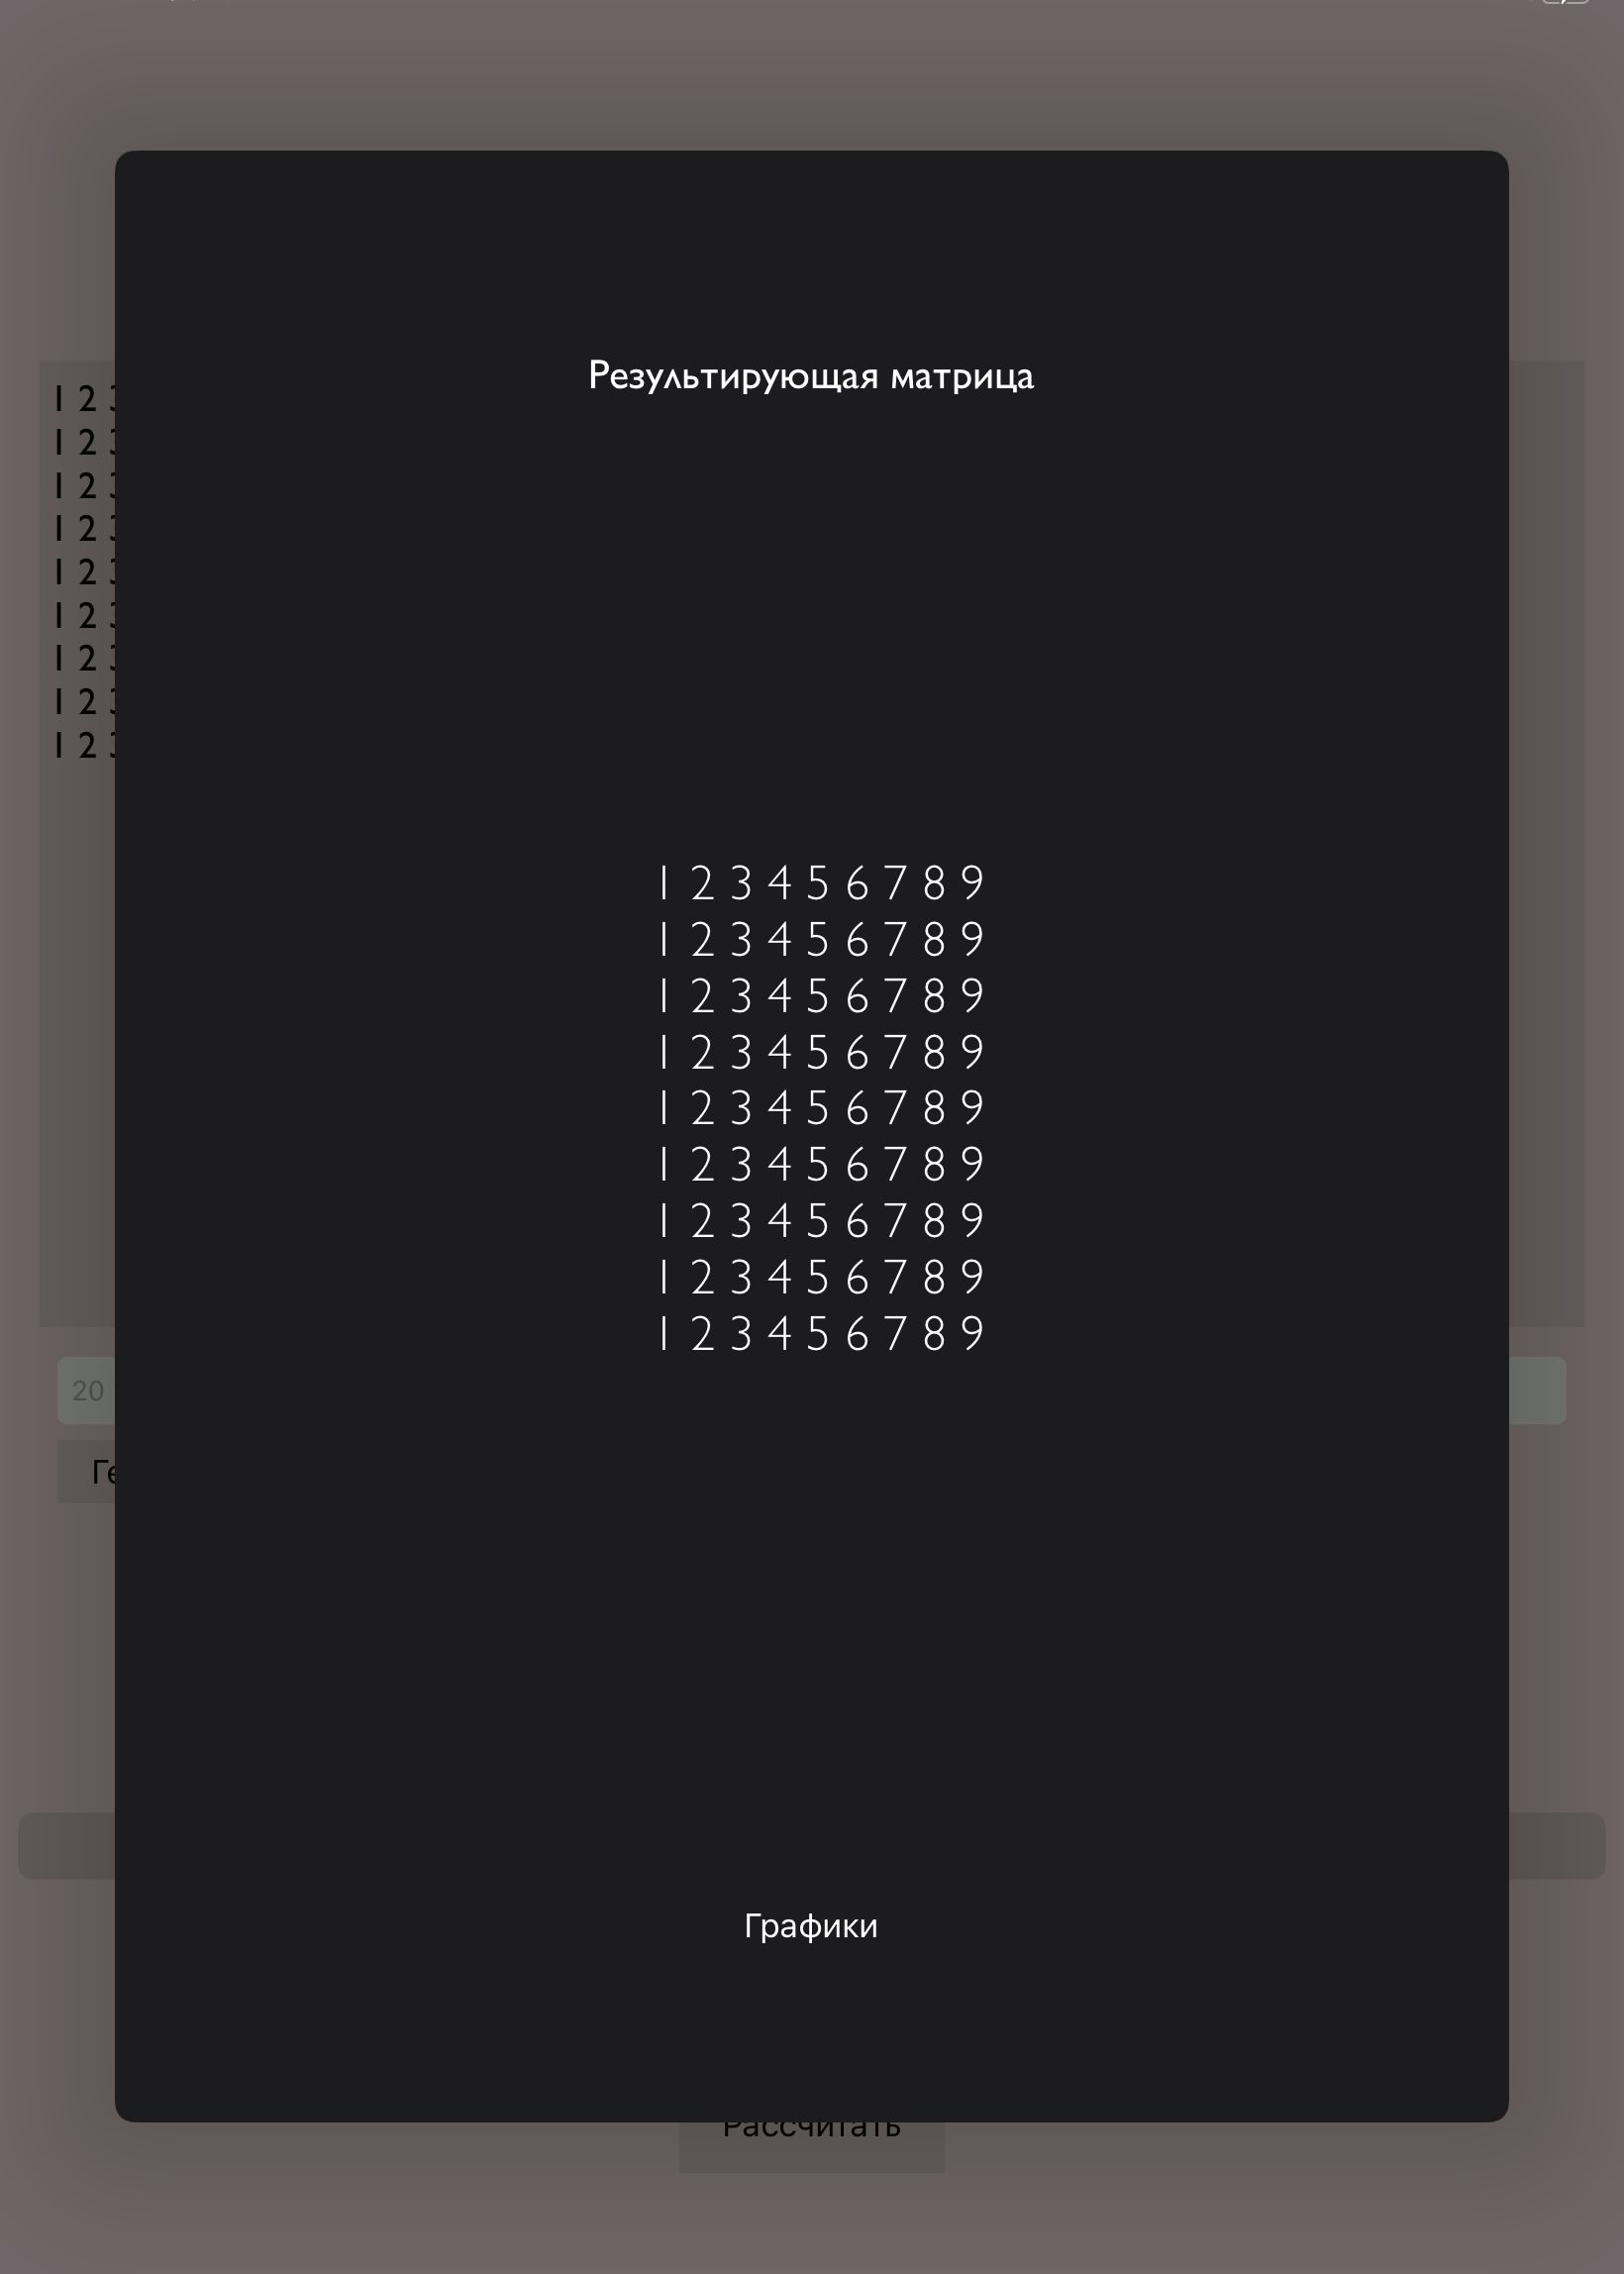
\includegraphics[scale=0.29]{img/работа.jpg}}
	\caption{Экран с результатом}
	\label{fig:работа}
\end{figure}

\begin{figure}[h!]
	\centering{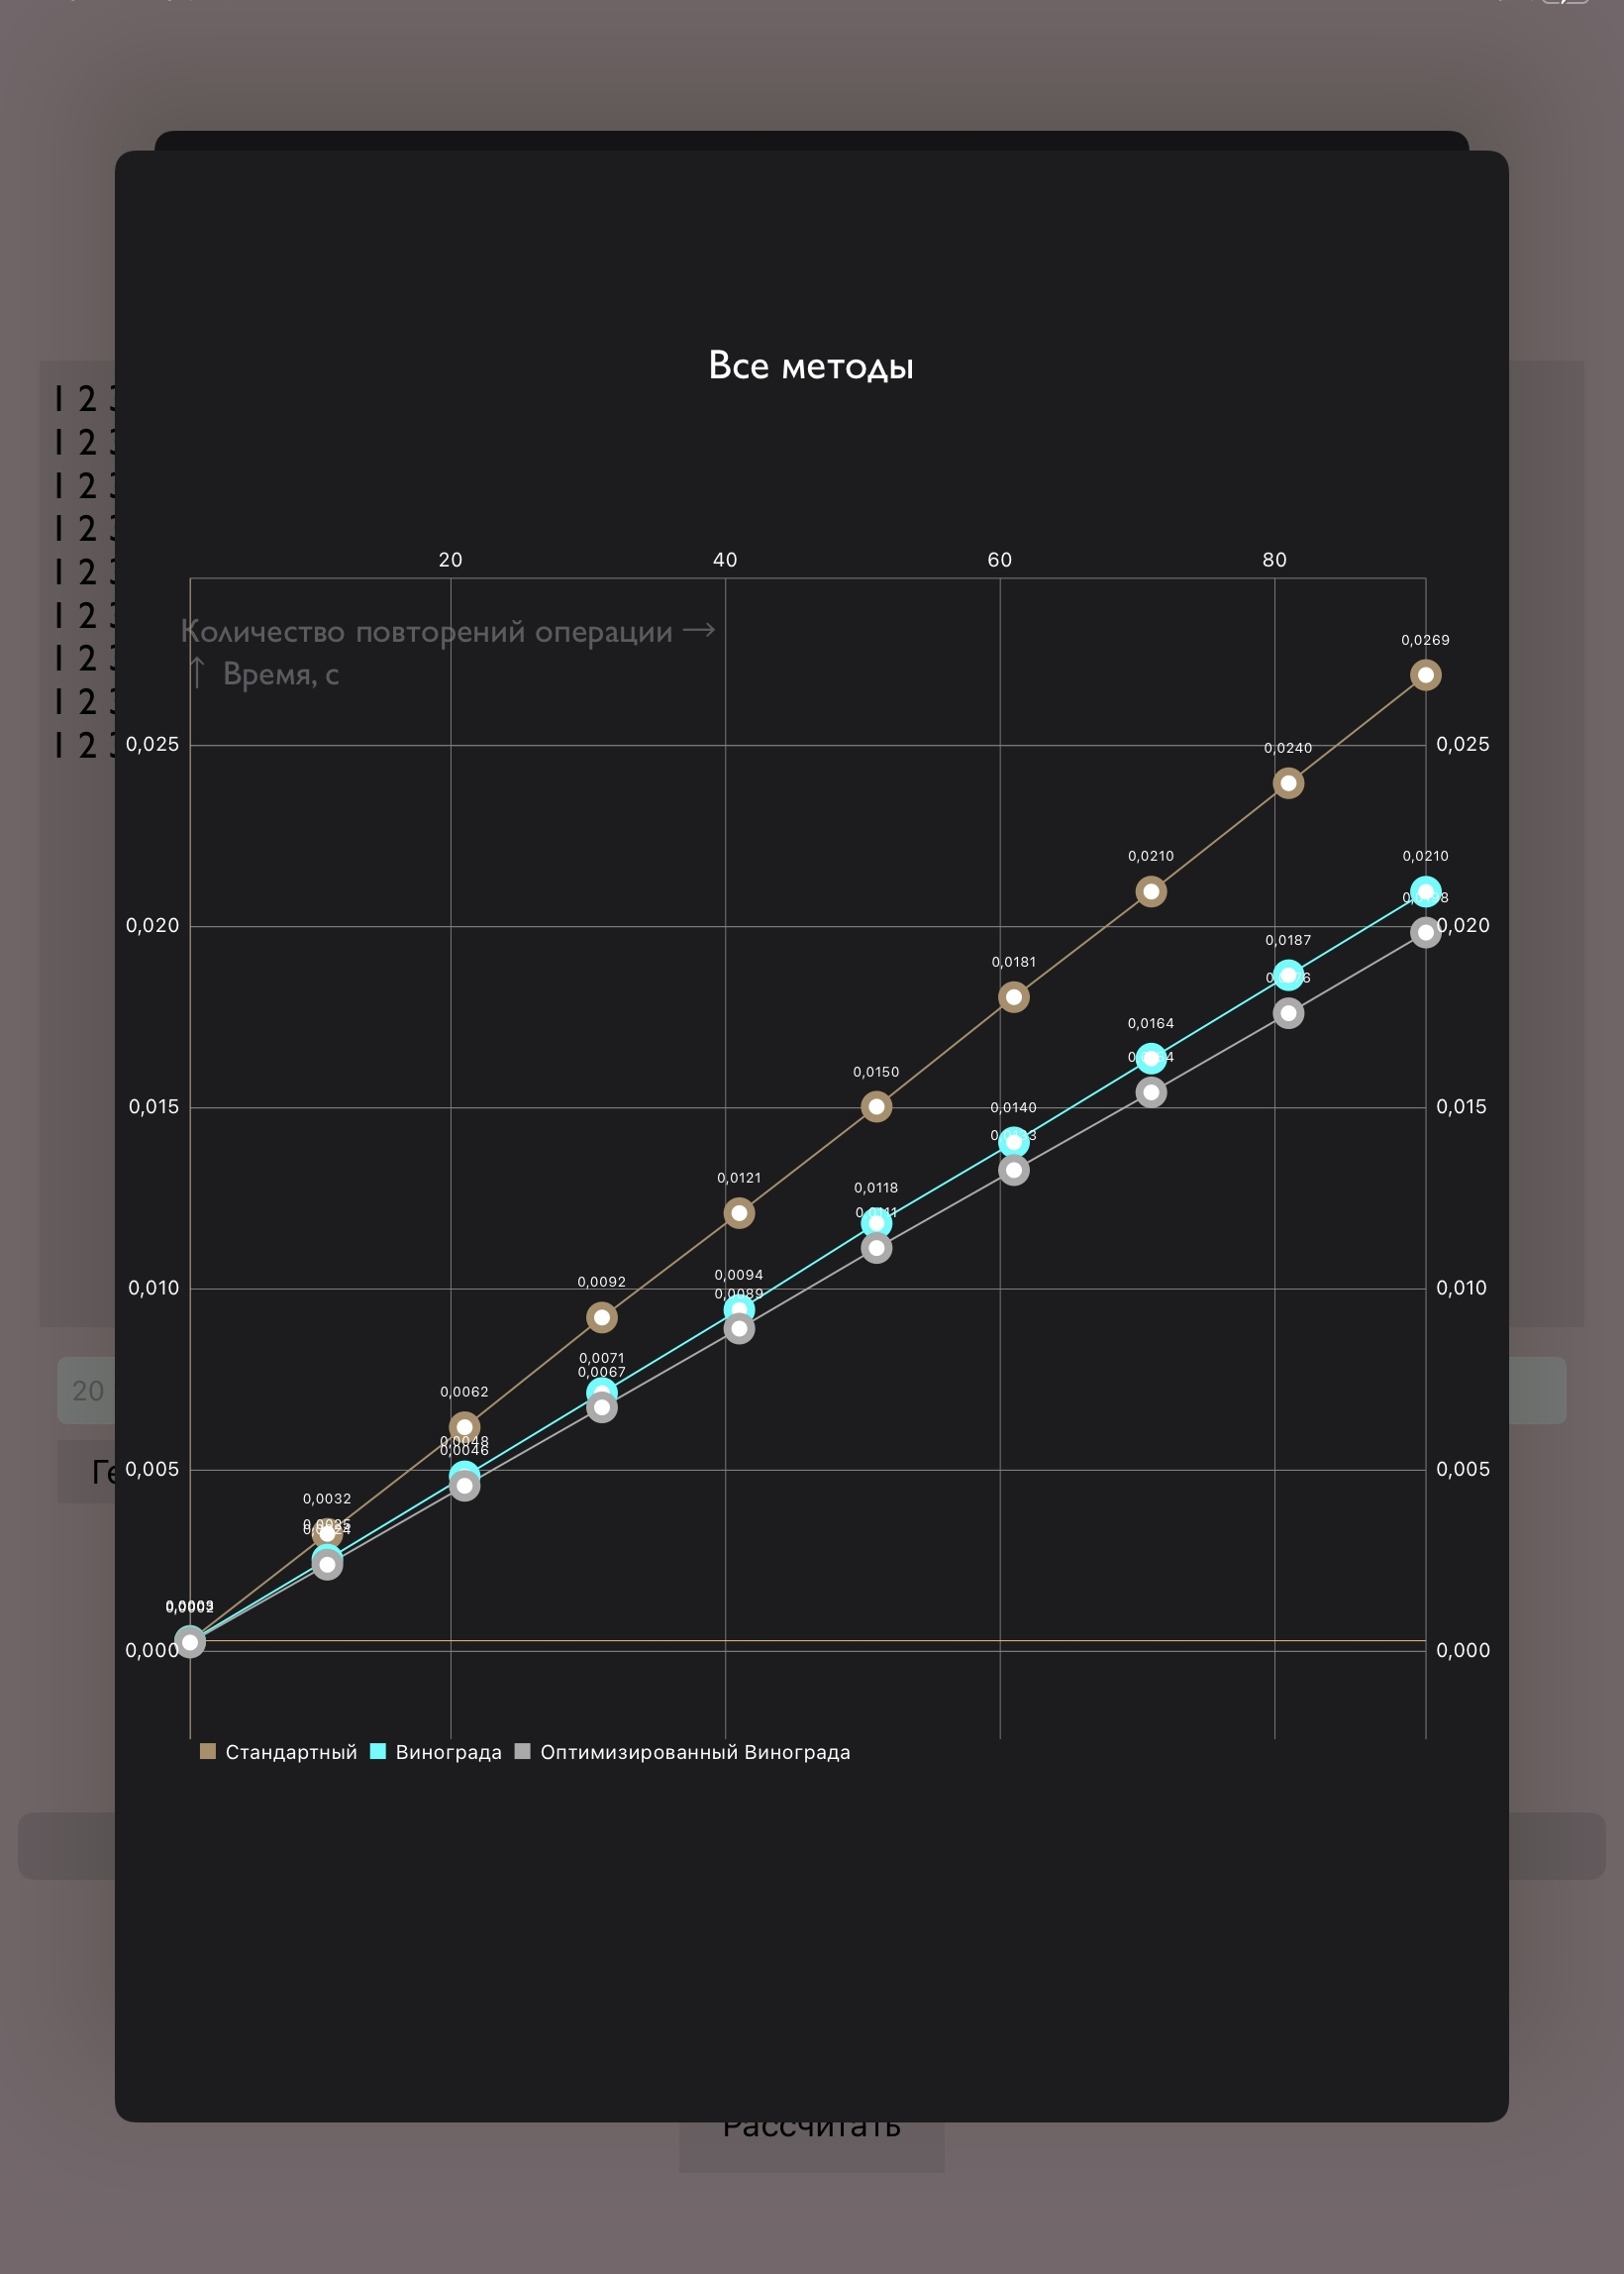
\includegraphics[scale=0.29]{img/график.jpg}}
	\caption{Экран с графиками}
	\label{fig:график}
\end{figure}

\section{Технические характеристики}



Технические характеристики устройства, на котором выполнялось тестирование:

\begin{itemize}
	\item операционная система: iOS 14.5;
	\item оперативная память: 4 Гб;
	\item процессор: Apple A14 Bionic 2990 МГц \cite{ipad};
\end{itemize}

Во время тестирования iPad не был подключен к другим устройствам и был включен в сеть питания.

\section{Время выполнения реализаций алгоритмов}

В таблице \ref{tab:time0} представлены замеры времени работы для каждого из алгоритмов для квадратных матриц небольшого размера (1-9). Здесь и далее: СА — стандартный алгоритм, АВ — алгоритм Винограда, ОАВ -- оптимизированный алгоритм Винограда. Время в микросекундах.

\begin{table}[h]
	\begin{center}
		\caption{\label{tab:time0}Результаты замеров времени алгоритмов при малых размерах матриц (микросекунды)}
		\begin{tabular}{|c|c|c|c|c|}
		\hline
		Размер & СА &  АВ & ОАВ \\
		\hline
		1  & 9.117 & 14.889 & 13.246\\
		\hline
		2  & 39.704 & 45.977 & 50.745\\
		\hline
		3  & 79.278 & 73.845 & 67.405 \\
		\hline
		4  & 148.618 & 150.349 & 115.306 \\
		\hline
		5  & 279.045 & 249.385 & 183.087 \\
		\hline
		6  & 359.754 & 367.953 & 265.140 \\
		\hline
		7  & 615.749 & 451.200 & 426.423 \\
		\hline
		8  & 883.049 & 602.657 & 541.336 \\
		\hline
		9  & 1194.958 & 825.197 & 799.224 \\
		\hline
		
		\end{tabular}
	\end{center}
\end{table}

Можно заметить, что при небольших размерах матриц стандартный алгоритм эффективнее алгоритма Винограда по времени. Однако с увеличение размеров матриц растет и эффективность работы алгоритма Винограда в сравнении со стандартным. Чтобы проследить разницу временных затрат стандартной реализации и реализации Винограда в двух вариациях, обратимся к матрицам большего размера. 

В таблицах \ref{tab:time1} и \ref{tab:time2} представлены замеры времени работы для каждого из алгоритмов. 
Замеры проводились для четных и нечетных квадратных матриц размером от 10 до 201. Высчитывалось среднее время при количестве повторений равном 50. Время в секундах.

\begin{table}[h]
	\begin{center}
		\caption{\label{tab:time1}Результаты замеров времени алгоритмов при четных размерах матриц (сек)}
		\begin{tabular}{|c|c|c|c|c|}
		\hline
		Размер & СА &  АВ & ОАВ \\
		\hline
		10  & 0.0017 & 0.0012 & 0.0010\\
		\hline
		20  & 0.0118 & 0.0076 & 0.0068\\
		\hline
		40  & 0.0953 & 0.0643 & 0.0616 \\
		\hline
		80  & 0.7289 & 0.4340 & 0.4054 \\
		\hline
		100  & 1.3709 & 0.9202 & 0.7693 \\
		\hline
		150  & 4.7042 & 2.6902 & 2.5413 \\
		\hline
		200  & 11.6528 & 6.3241 & 5.9507 \\
		\hline
		
		\end{tabular}
	\end{center}
\end{table}

\begin{table}[h]
	\begin{center}
		\caption{\label{tab:time2}Результаты замеров времени алгоритмов при нечетных размерах матриц (сек)}
		\begin{tabular}{|c|c|c|c|c|}
		\hline
		Размер & СА &  АВ & ОАВ \\
		\hline
		11  & 0.0020 & 0.0013 & 0.0014\\
		\hline
		21  & 0.0133 & 0.0088 & 0.0079\\
		\hline
		41  & 0.0915 & 0.0540 & 0.0518 \\
		\hline
		81  & 0.7135 & 0.4110 & 0.3831 \\
		\hline
		101  & 1.6259 & 0.9673 & 1.1453 \\
		\hline
		151  & 5.5601 & 2.9469 & 2.7519 \\
		\hline
		201  & 12.1178 & 7.2646 & 6.7645 \\
		\hline		
		\end{tabular}
	\end{center}
\end{table}


\section*{Вывод}
При увеличении размера матриц, увеличивается и эффективность работы алгоритма Винограда в сравнении со стандартным алгоритмом. В среднем первый алгоритм работает быстрее в 1.7 раз. Оптимизированная реализация алгоритма Винограда также позволяет уменьшить время работы при больших размерностях. 

